\documentclass[12pt, letter]{exam}
\usepackage[utf8]{inputenc}
\usepackage[T1]{fontenc}
\usepackage[spanish]{babel}
\usepackage[autostyle,spanish=mexican]{csquotes}
\usepackage{amsmath}
\usepackage{amsthm}
\usepackage{physics}
\usepackage{tikz}
\usepackage{float}
\usepackage{siunitx}
\usepackage{multicol}
\usepackage[left=2.00cm, right=2.00cm, top=2.00cm, 
     bottom=2.00cm]{geometry}
\usepackage{pdfpages}

% \renewcommand{\questionlabel}{\thequestion}
\decimalpoint

\setlength{\belowdisplayskip}{-0.5pt}

\usepackage{tasks}
\settasks{
    label=\Alph*), 
    label-align=left,
    item-indent={20pt}, 
    column-sep={4pt},
    label-width={16pt},
}

\sisetup{per-mode=symbol}
\footer{}{\thepage}{}

\begin{document}
\includepdf[pages={1}]{Caratula_Examen_Parcial_02_PU_Fisica_4_01.pdf}

\newpage

\begin{questions}
    
    \section{Naturaleza de la luz.}

    \question ¿Cuáles son las características de la luz que se cumplen tanto en la teoría corpuscular de la luz y la teoría ondulatoria?
    \begin{parts}
        \part Reflexión, Resonancia, Propagación rectilínea.
        \part Propagación rectilínea, Reflexión, Refracción.
        \part Refracción, Reverberación, Reflexión.
        \part Refracción, Efecto Doppler, Reflexión.
    \end{parts}
    \question Nombre del científico que propuso que la luz es un fenómeno ondulatorio semejante al sonido.
    \begin{tasks}(4)
        \task Isaac \\ Newton.
        \task James \\ Maxwell.
        \task Christian \\ Huygens.
        \task Willebrord \\ Snell.
    \end{tasks}
    \question Completa la frase con la palabra que hace falta. Un cuerpo \rule{2cm}{0.1mm} deja pasar la luz, pero la difunde de tal manera que las cosas no pueden ser distinguidas claramente a través de él.
    \begin{tasks}(4)
        \task Transparente.
        \task Opaco.
        \task Translúcido.
        \task Reflejante.
    \end{tasks}
    
    \section{Óptica geométrica.}

    \question \label{Problema_01} \textbf{Ejercicio de ejecución: } El haz de una linterna incide sobre la superficie de un panel
    de vidrio $(n = 1.56)$ en un ángulo de \ang{63} con la normal. ¿Cuál es el ángulo de refracción?
    \begin{tasks}(4)
        \task \ang{34;49;51}
        \task \ang{34;25;14}
        \task \ang{89;10;10}
        \task \ang{57;11;58}
    \end{tasks}
    \question Tomando el enunciado anterior de la linterna, ahora considera que el haz de luz incide sobre la superficie de otro material cuyo índice es $n_{2} = 1.2$, en comparación al ángulo de refracción con el vidrio $\theta_{n1}$, ¿cómo será el ángulo de refracción $\theta_{n2}$ en la otra superficie?
    \begin{tasks}(4)
        \task Mayor que $\theta_{n1}$
        \task Menor que $\theta_{n1}$
        \task Son iguales.
        \task La mitad de $\theta_{n1}$
    \end{tasks}
    \question La refracción de la luz consiste en la desviación que sufren los rayos luminosos cuando llegan a la superficie de separación entre dos sustancias o medios de diferente \rule{2.5cm}{0.1mm}.
    \begin{tasks}(4)
        \task Volumen.
        \task Grosor.
        \task Densidad.
        \task Peso.
    \end{tasks}
    \question De la ley de Snell se nos pide obtener el índice de refracción del medio $b$, ¿cuál es la expresión que nos resuelve el problema?
    \begin{tasks}(4)
        \task $n_{b} = \dfrac{\text{sen} \, b}{n_{a} \, \text{sen} \, a}$
        \task $n_{b} = \dfrac{n_{a} \, \text{sen} \, b}{\text{sen} \, a}$
        \task $n_{b} = \dfrac{n_{a} \, \text{sen} \, a}{\text{sen} \, b}$
        \task $n_{b} = \dfrac{\text{sen} \, a}{n_{a} \, \text{sen} \, b}$
    \end{tasks}

    \section{Lentes delgadas.}

    \question Las lentes \rule{2.5cm}{0.1mm} son aquellas cuyo espesor va disminuyendo del centro hacia los bordes, hablamos de las lentes:
    \begin{tasks}(4)
        \task Divergentes.
        \task Cilíndricas.
        \task Convergentes.
        \task Esféricas.
    \end{tasks}
    \question La propiedad del centro óptico de la lente nos dice que en ese punto la desviación de un rayo de luz es:
    \begin{tasks}(4)
        \task Máxima.
        \task Perpendicular al \\ eje principal.
        \task Nula.
        \task Infinita.
    \end{tasks}
    \question Cuando hablamos del punto donde se cruzan los rayos que llegan a la lente en forma paralela al eje principal, estamos hablando de:
    \begin{tasks}(4)
        \task Foco \\ principal.
        \task Centro \\ geométrico.
        \task Eje \\ principal.
        \task Plano \\ central
    \end{tasks}
    \question Revisa con cuidado la siguiente imagen e identifica las siguientes lentes.
    \begin{figure}[H]
        \centering
        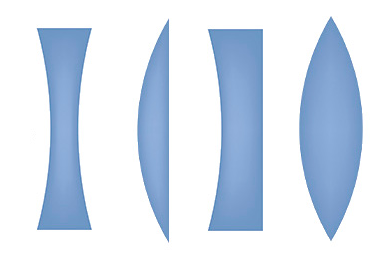
\includegraphics[scale=2]{Imagenes/Arreglo_Lentes_01.png}
    \end{figure}
    \begin{tasks}(4)
        \task +, - , +, - 
        \task +, + , -, - 
        \task -, + , +, - 
        \task -, + , -, + 
    \end{tasks}
    \question De la convención de signos para las lentes delgadas:  La distancia del objeto $d_{0}$ es \rule{2cm}{0.1mm} si el objeto está en el lado de la lente de donde proviene la luz:
    \begin{tasks}(4)
        \task Positiva.
        \task Cero.
        \task Infinita.
        \task Negativa.
    \end{tasks}
    \question De la convención de signos para las lentes delgadas:  La distancia de la imagen $d_{i}$ es \rule{2cm}{0.1mm} para una imagen virtual.
    \begin{tasks}(4)
        \task Negativa.
        \task Positiva.
        \task Infinita.
        \task Cero.
    \end{tasks}
    \question \label{Problema_02} \textbf{Ejercicio de ejecución. } Un objeto de \SI{15}{\centi\meter} se coloca a \SI{50}{\centi\meter} de una lente positiva que tiene una distancia focal de \SI{20}{\centi\meter}. ¿De qué tamaño es la imagen?
    \begin{tasks}(4)
        \task \SI{25}{\centi\meter}
        \task \SI{10}{\centi\meter}
        \task \SI{5}{\centi\meter}
        \task \SI{33}{\centi\meter}
    \end{tasks}
    \question \label{Problema_03} \textbf{Ejercicio de ejecución: } ¿Cuál es la potencia de una lente con \SI{23.5}{\centi\meter} de distancia focal?
    \begin{tasks}(4)
        \task \num{4.25} Dioptrías
        \task \num{-5.25} Dioptrías
        \task \num{10.25} Dioptrías
        \task \num{-0.25} Dioptrías
    \end{tasks}

    \section{El ojo y la visión.}

    \question El siguiente esquema representa un ojo humano, ¿cómo se denomina al caso en términos de anomalías/normalidad de la visión?
    \begin{figure}[H]
        \centering
        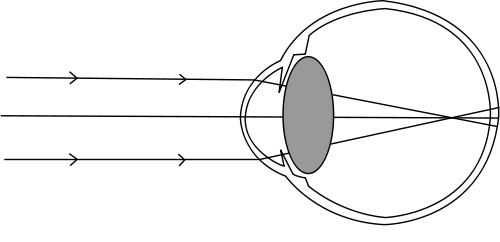
\includegraphics[scale=0.3]{Imagenes/Defectos_Vision_03.png}
    \end{figure}
    \begin{tasks}(4)
        \task Ojo miope.
        \task Ojo emétrope.
        \task Ojo hipermétrope.
        \task Ojo astigmata.
    \end{tasks}
    \question El siguiente esquema representa en términos de anomalías/normalidad de la visión?
    \begin{figure}[H]
        \centering
        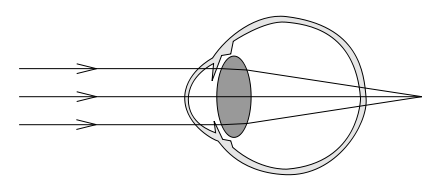
\includegraphics[scale=0.4]{Imagenes/Defectos_Vision_05.png}
    \end{figure}
    \begin{tasks}(4)
        \task Ojo hipermétrope.
        \task Ojo miope.
        \task Ojo astigmata.
        \task Ojo emétrope.
    \end{tasks}
    \question El ojo présbita: suele ser un ojo \enquote{cansado} debido a que la facultad de \rule{2cm}{0.1mm} ha disminuido.
    \begin{tasks}(4)
        \task Visión binocular.
        \task Densidad del \\ humor vítreo.
        \task Presión interna.
        \task Acomodación \\ del cristalino.
    \end{tasks}
    \question  La \rule{2cm}{0.1mm} es la capacidad de utilizar ambos ojos de manera coordinada y simultánea para percibir una sola imagen tridimensional del entorno.
    \begin{tasks}(4)
        \task Visión monocular.
        \task Visión periférica.
        \task Visión 20/20.
        \task Visión binocular.
    \end{tasks}
    \question Cuando decimos que se trata de una enfermedad degenerativa provocada por la alteración en las fibras de colágeno que componen el estroma (la parte más gruesa de la córnea), provocando una pérdida paulatina de la visión. Hablamos de:
    \begin{tasks}(4)
        \task Escotoma.
        \task Glaucoma.
        \task Queratocono.
        \task Cataratas.
    \end{tasks}
\end{questions}

\newpage

\textbf{\huge{Formulario.}}
\begin{table}[H]
    \centering
    \setlength{\tabcolsep}{40pt}
    \renewcommand{\arraystretch}{2.5}
    \begin{tabular}{c  c}
        \multicolumn{2}{c}{Óptica geométrica} \\
        $n = \dfrac{\text{sen} \, i}{\text{sen} \, i}$ & $n_{a} \, \text{sen} \,  a = n_{b} \, \text{sen} \,  b$ \\ \hline
        \multicolumn{2}{c}{Lentes delgadas} \\
        $\dfrac{1}{f} = \dfrac{1}{d_{o}} + \dfrac{1}{d_{i}}$ (lente convergente) & $- \dfrac{1}{f} = \dfrac{1}{d_{o}} - \dfrac{1}{d_{i}}$ (lente divergente) \\
        $m = - \dfrac{d_{i}}{d_{o}} = \dfrac{h_{i}}{h_{o}}$ & $\text{Potencia } = \dfrac{1}{f} \quad f \text{ en } \unit{\meter}$ \\ \hline
\end{tabular}
\end{table}

En este espacio deberás de incluir el desarrollo completo de los Problemas de Ejecución. Recuerda que si no se tiene el desarrollo, el problema no aportará puntaje aunque se tenga la respuesta correcta.

\vspace*{0.5cm}
Solución al Problema de Ejecución \ref{Problema_01}:

\vspace*{4cm}
\rule{0.9\textwidth}{0.3mm}

Solución al Problema de Ejecución \ref{Problema_02}:

\vspace*{4.5cm}
\rule{0.9\textwidth}{0.3mm}

Solución al Problema de Ejecución \ref{Problema_03}:


\end{document}